%%%%%%%%%%%%%%%%%%%%%%%%%%%%%%%%%%%%%%%%%
% Beamer Presentation
% LaTeX Template
% Version 2.0 (March 8, 2022)
%
% This template originates from:
% https://www.LaTeXTemplates.com
%
% Author:
% Vel (vel@LaTeXTemplates.com)
%
% License:
% CC BY-NC-SA 4.0 (https://creativecommons.org/licenses/by-nc-sa/4.0/)
%
%%%%%%%%%%%%%%%%%%%%%%%%%%%%%%%%%%%%%%%%%

%----------------------------------------------------------------------------------------
%\tPACKAGES AND OTHER DOCUMENT CONFIGURATIONS
%----------------------------------------------------------------------------------------

\documentclass[
    11pt,
    %t,
    %aspectratio=169,
]{beamer}

\graphicspath{{assets/}{./}}

\usepackage{booktabs}
\usepackage{amsmath}
\usepackage{tikz}
\usepackage{pgfplots}

\pgfplotsset{compat=1.18}

%----------------------------------------------------------------------------------------
%\tSELECT LAYOUT THEME
%----------------------------------------------------------------------------------------

%\usetheme{default}
%\usetheme{AnnArbor}
%\usetheme{Antibes}
%\usetheme{Bergen}
%\usetheme{Berkeley}
%\usetheme{Berlin}
%\usetheme{Boadilla}
%\usetheme{CambridgeUS}
%\usetheme{Copenhagen}
%\usetheme{Darmstadt}
%\usetheme{Dresden}
%\usetheme{Frankfurt}
%\usetheme{Goettingen}
%\usetheme{Hannover}
%\usetheme{Ilmenau}
%\usetheme{JuanLesPins}
%\usetheme{Luebeck}
\usetheme{Madrid}
%\usetheme{Malmoe}
%\usetheme{Marburg}
%\usetheme{Montpellier}
%\usetheme{PaloAlto}
%\usetheme{Pittsburgh}
%\usetheme{Rochester}
%\usetheme{Singapore}
%\usetheme{Szeged}
%\usetheme{Warsaw}

%----------------------------------------------------------------------------------------
%\tSELECT COLOR THEME
%----------------------------------------------------------------------------------------

%\usecolortheme{albatross}
%\usecolortheme{beaver}
%\usecolortheme{beetle}
%\usecolortheme{crane}
%\usecolortheme{dolphin}
%\usecolortheme{dove}
%\usecolortheme{fly}
%\usecolortheme{lily}
%\usecolortheme{monarca}
%\usecolortheme{seagull}
%\usecolortheme{seahorse}
%\usecolortheme{spruce}
%\usecolortheme{whale}
%\usecolortheme{wolverine}

%----------------------------------------------------------------------------------------
%\tSELECT FONT THEME & FONTS
%----------------------------------------------------------------------------------------

\usefonttheme{default}
%\usefonttheme{serif}
%\usefonttheme{structurebold}
%\usefonttheme{structureitalicserif}
%\usefonttheme{structuresmallcapsserif}

%------------------------------------------------

%\usepackage{mathptmx}
\usepackage{palatino}

%\usepackage{helvet}
\usepackage[default]{opensans}
%\usepackage[default]{FiraSans}
%\usepackage[default]{lato}

%----------------------------------------------------------------------------------------
%\tSELECT INNER THEME
%----------------------------------------------------------------------------------------

%\useinnertheme{default}
\useinnertheme{circles}
%\useinnertheme{rectangles}
%\useinnertheme{rounded}
%\useinnertheme{inmargin}

%----------------------------------------------------------------------------------------
%\tSELECT OUTER THEME
%----------------------------------------------------------------------------------------

%\useoutertheme{default}
%\useoutertheme{infolines}
%\useoutertheme{miniframes}
%\useoutertheme{smoothbars}
%\useoutertheme{sidebar}
%\useoutertheme{split}
%\useoutertheme{shadow}
%\useoutertheme{tree}
%\useoutertheme{smoothtree}

%\setbeamertemplate{footline}
%\setbeamertemplate{footline}[page number]

%\setbeamertemplate{navigation symbols}{}

%----------------------------------------------------------------------------------------
%\tPRESENTATION INFORMATION
%----------------------------------------------------------------------------------------

\title[Power Flow Analysis]{Power Flow Analysis}

\subtitle{A Linear Solution to Economic Electric Grid Scheduling}

\author[Sa'ad \and Max \and Buck \and Tim]{Sa'ad Farooq \and Maxwell Fang \and Buck Chen \and Timothy Zheng}

\institute[UW]{Faculty of Mathematics \\ \smallskip \textit{Department of Combinatorics \& Optimization}}

\date[\today]{Final Project for CO 370 - Deterministic OR Models \\ \today}

%----------------------------------------------------------------------------------------

\begin{document}

%----------------------------------------------------------------------------------------
%\tTITLE SLIDE
%----------------------------------------------------------------------------------------

\begin{frame}
    \titlepage
\end{frame}

%----------------------------------------------------------------------------------------
%\tTABLE OF CONTENTS SLIDE
%----------------------------------------------------------------------------------------

\begin{frame}
    \frametitle{The US Power Market}
    \begin{center}
        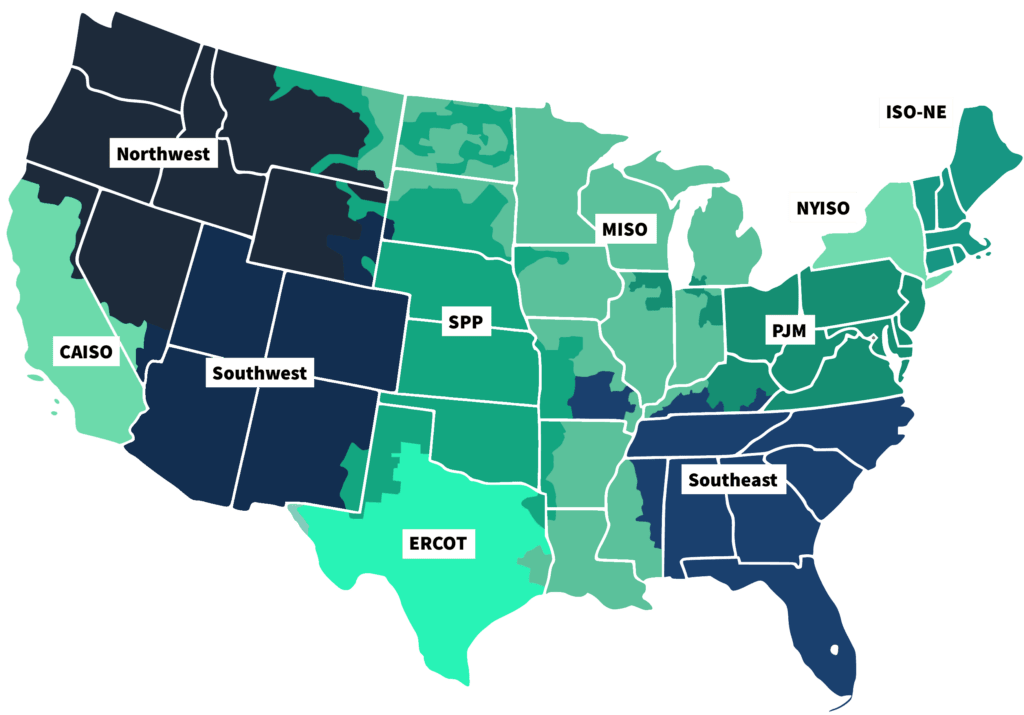
\includegraphics[width=\textwidth,height=0.75\textheight,keepaspectratio]{assets/ISO-map.png}
    \end{center}
\end{frame}

\begin{frame}
    \frametitle{The US Power Market}
    \begin{center}
        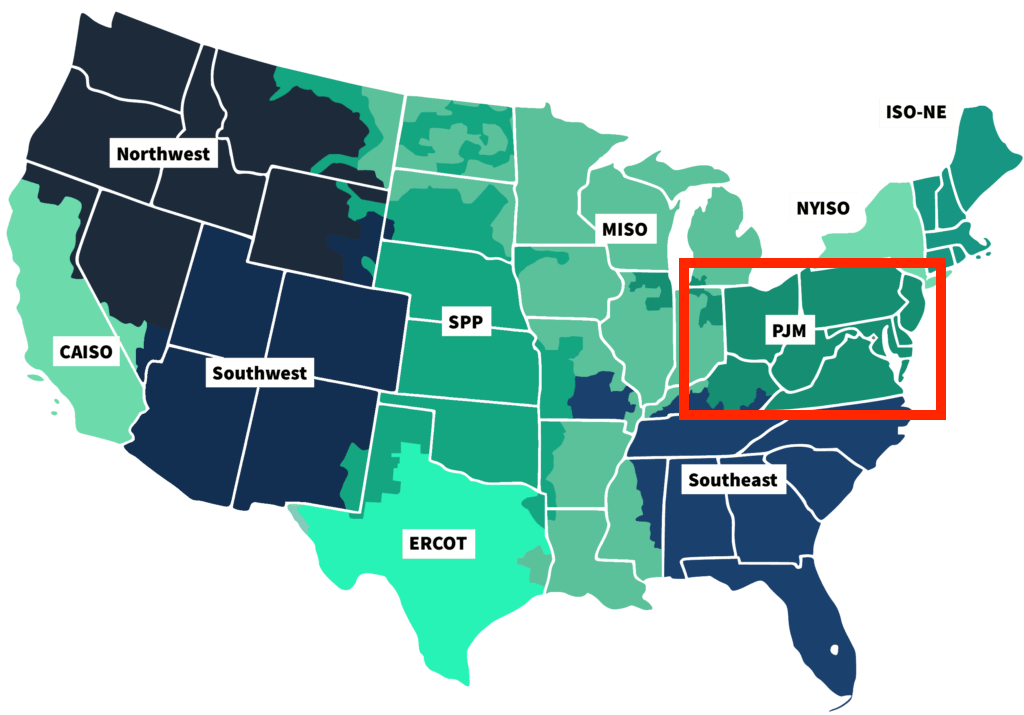
\includegraphics[width=\textwidth,height=0.82\textheight,keepaspectratio]{assets/PJM.png}
    \end{center}
\end{frame}

\begin{frame}
    \frametitle{The US Power Market}
    \begin{center}
        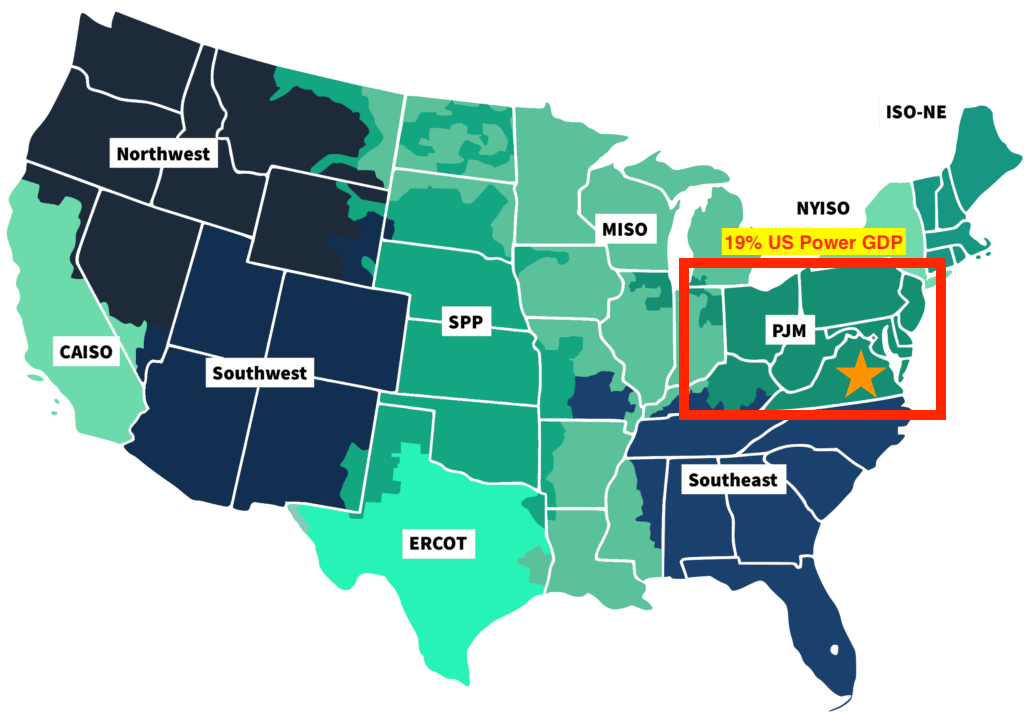
\includegraphics[width=\textwidth,height=0.82\textheight,keepaspectratio]{assets/virginia.png}
    \end{center}
\end{frame}

\begin{frame}
    \frametitle{The US Power Market}
    \begin{center}
        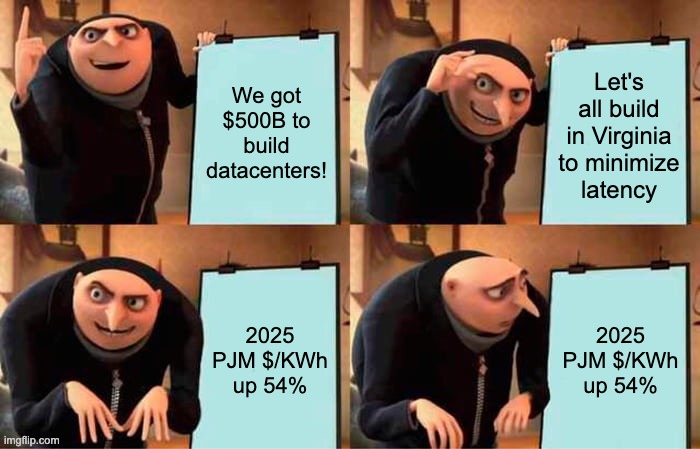
\includegraphics[width=\textwidth,height=0.68\textheight,keepaspectratio]{assets/meme.jpg}
    \end{center}

    {\footnotesize Source: \href{https://www.utilitydive.com/news/pjm-capacity-energy-market-reliability-monitoring-analytics/814647/}{Utility Dive on PJM capacity markets}}
\end{frame}

\begin{frame}
    \frametitle{Presentation Overview}
    \tableofcontents
\end{frame}

%----------------------------------------------------------------------------------------
%\tPRESENTATION BODY SLIDES
%----------------------------------------------------------------------------------------

\section{Problem Description}

\begin{frame}
    \frametitle{The North American Power Grid}
    \small

    \begin{center}
        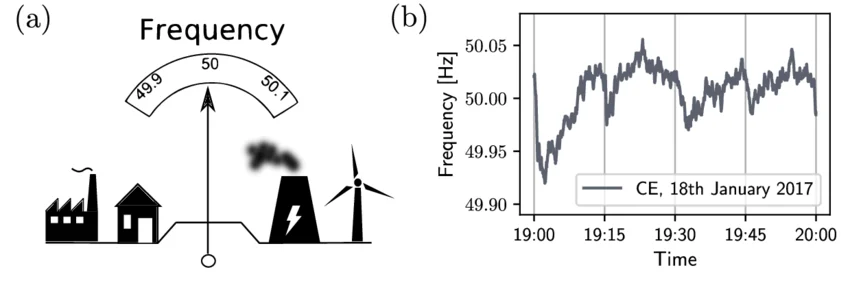
\includegraphics[width=\textwidth,height=0.4\textheight,keepaspectratio]{assets/grid-frequency.png}
    \end{center}

    \begin{itemize}
        \item The \alert{power grid} is a network of \alert{generators}, \alert{loads}, and \alert{power lines} that are constantly trading with each other to supply electricity.
        \item \textit{Unlike other markets}, power is delivered instantly and is subject to transmission and power-balance constraints due to physical limits.
        \item \alert{Regional Transmission Operators (RTOs)} ensure economic dispatch of power by telling participants how much power to use/generate.
    \end{itemize}
\end{frame}

\begin{frame}
    \frametitle{Aside: Electricity 101}
    \small

    \begin{columns}[T,onlytextwidth]
        \begin{column}{0.7\textwidth}
            \begin{itemize}
                \item Electricity doesn't care about what you want.
                \item 1 MW injected into a single point in the grid will \alert{spread out} across the network and intermingle with power from other generators.
                \item The amount of power that flows through each transmission line is defined by which \alert{gens} and \alert{loads} are authorized to inject/withdraw.
            \end{itemize}
        \end{column}
        \begin{column}{0.28\textwidth}
            \vspace{-0.3em}
            \begin{center}
                
\includegraphics[width=\linewidth]{assets/image.png}
            \end{center}
        \end{column}
    \end{columns}

    \vspace{0.2em}
    \begin{block}{Takeaway 1}
        Electricity can't easily be "routed" through transmission lines. It flows relative to physical conditions of the grid. The percentage of each MW that goes through each transmission line is its \alert{shift factor}.
    \end{block}
\end{frame}

\begin{frame}
    \frametitle{The Market-Clearing Problem}
    \small

    \begin{itemize}
        \item In the \alert{Day-Ahead (DA) market}, generators submit offers and loads submit bids for the next 24 hours.
        \item The RTO \alert{clears} the auction to obtain a feasible generation and consumption schedule maximizing revenue (to maximize grid utilization).
        \item Additionally, the RTO places a \alert{(N-1) contingency constraint}, requiring any cleared solution to also be feasible if any one line goes down. 
        \item We study a DC approximation of optimal power flow, then extend the model to clear \alert{Financial Transmission Rights (FTRs)}.

        \vspace{0.2em}
        \begin{block}{Takeaway 2}
            There are many feasible (and even more) infeasible solutions to the DA clearing problem. We strive to find the one that clears the most power.
        \end{block}
    \end{itemize}
\end{frame}

%------------------------------------------------

\section{Small Example}

\begin{frame}
    \frametitle{3-Node Grid Example}

    \begin{columns}[T,totalwidth=\textwidth]
        \begin{column}{0.4\textwidth}
            \begin{center}
            \resizebox{\linewidth}{!}{%
            \begin{tikzpicture}[every node/.style={font=\normalsize}]
              \node[draw, circle, minimum size=1.2cm] (A) at (0,2.8) {A};
              \node[draw, circle, minimum size=1.2cm] (B) at (6.6,2.8) {B};
              \node[draw, circle, minimum size=1.2cm] (C) at (3.3,0) {C};

              \draw[thick] (A) -- (B);
              \draw[thick] (B) -- (C);
              \draw[thick] (A) -- (C);

              \node[align=left] at (-2.3,2.9) {Gen 1\\Load 1};
              \node[align=left] at (8.8,2.9) {Gen 2};
              \node[align=center] at (3.3,-1.4) {Gen 3\\Load 2, Load 3};
            \end{tikzpicture}%
            }
            \end{center}

            \vspace{0.5em}
            \textbf{Line limits}
            \begin{center}
            \scriptsize
            \resizebox{0.9\linewidth}{!}{%
            \begin{tabular}{lc}
                \toprule
                Line & Limit \\
                \midrule
                $A \rightarrow C$ & 3 MW \\
                $A \rightarrow B$ & 3 MW \\
                $B \rightarrow C$ & 3 MW \\
                \bottomrule
            \end{tabular}%
            }
            \end{center}
        \end{column}
        \begin{column}{0.56\textwidth}
            \textbf{Supply offers}
            \begin{center}
            \scriptsize
            \resizebox{\linewidth}{!}{%
            \begin{tabular}{lccc}
                \toprule
                Generator & Node & Offer & Max MW \\
                \midrule
                Gen 1 & $A$ & \$5.00 & 2.0 \\
                Gen 2 & $B$ & \$10.00 & 10.0 \\
                Gen 3 & $C$ & \$7.50 & 0.5 \\
                \bottomrule
            \end{tabular}%
            }
            \end{center}

            \vspace{0.4em}
            \textbf{Demand bids}
            \begin{center}
            \scriptsize
            \resizebox{\linewidth}{!}{%
            \begin{tabular}{lccc}
                \toprule
                Load & Node & Demand & Bid \\
                \midrule
                Load 1 & $A$ & 1.0 & \$6.50 \\
                Load 2 & $C$ & 2.0 & \$7.50 \\
                Load 3 & $C$ & 1.5 & \$10.00 \\
                \bottomrule
            \end{tabular}%
            }
            \end{center}
        \end{column}
    \end{columns}
\end{frame}

\begin{frame}
    \frametitle{Base Case Clearing}

    \small

    \begin{columns}[T,onlytextwidth]
        \begin{column}{0.52\textwidth}
            \textbf{Shift factors for source $A$, sink $C$}

            \begin{center}
            \begin{tabular}{ccc}
                \toprule
                $A \rightarrow B$ & $B \rightarrow C$ & $A \rightarrow C$ \\
                \midrule
                0.1 & 0.1 & 0.9 \\
                \bottomrule
            \end{tabular}
            \end{center}

            \vspace{0.2em}
            1 MW injected at $A$ and withdrawn at $C$ flows as follows:

            \begin{center}
            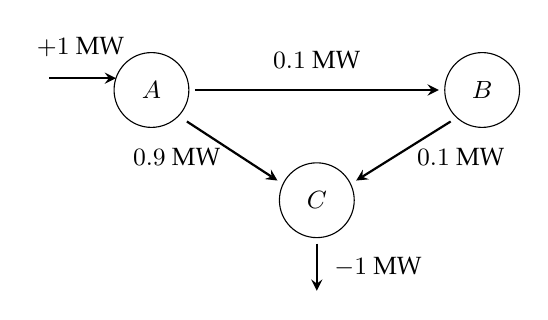
\begin{tikzpicture}[>=stealth, every node/.style={font=\small}]
                \node[draw, circle, minimum size=0.95cm] (A) at (0,1.4) {$A$};
                \node[draw, circle, minimum size=0.95cm] (B) at (4.2,1.4) {$B$};
                \node[draw, circle, minimum size=0.95cm] (C) at (2.1,0) {$C$};

                \draw[->, thick] (-1.3,1.55) -- (-0.45,1.55);
                \node[above] at (-0.9,1.7) {$+1$ MW};

                \draw[->, thick] (0.55,1.4) -- (3.65,1.4);
                \node[above] at (2.1,1.55) {$0.1$ MW};

                \draw[->, thick] (0.45,1.0) -- (1.6,0.25);
                \node[left] at (1.0,0.55) {$0.9$ MW};

                \draw[->, thick] (3.8,1.0) -- (2.6,0.25);
                \node[right] at (3.25,0.55) {$0.1$ MW};

                \draw[->, thick] (2.1,-0.55) -- (2.1,-1.15);
                \node[right] at (2.2,-0.85) {$-1$ MW};
            \end{tikzpicture}
            \end{center}
        \end{column}
        \begin{column}{0.45\textwidth}
            \textbf{One feasible solution}

            \begin{center}
            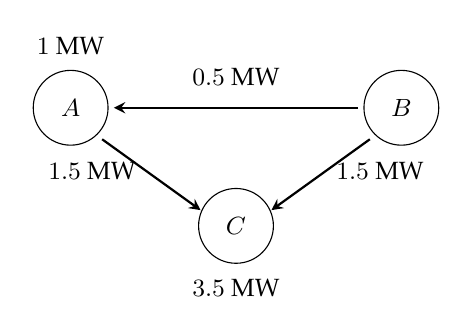
\begin{tikzpicture}[>=stealth, every node/.style={font=\small}]
                \node[draw, circle, minimum size=0.95cm] (A) at (0,1.5) {$A$};
                \node[draw, circle, minimum size=0.95cm] (B) at (4.2,1.5) {$B$};
                \node[draw, circle, minimum size=0.95cm] (C) at (2.1,0) {$C$};

                \node[above] at (0,2.05) {$1$ MW};
                \node[below] at (2.1,-0.55) {$3.5$ MW};

                \draw[->, thick] (3.65,1.5) -- (0.55,1.5);
                \node[above] at (2.1,1.65) {$0.5$ MW};

                \draw[->, thick] (0.4,1.1) -- (1.65,0.2);
                \node[left] at (0.95,0.7) {$1.5$ MW};

                \draw[->, thick] (3.8,1.1) -- (2.55,0.2);
                \node[right] at (3.25,0.7) {$1.5$ MW};
            \end{tikzpicture}
            \end{center}

            {\scriptsize
            \begin{itemize}
                \item Net loads: $A = 1$ MW, $C = 3.5$ MW.
                \item Gen 1 produces 2 MW.
                \item Gen 2 produces 2 MW.
                \item Gen 3 produces 0.5 MW.
                \item All loads are fully filled.
            \end{itemize}
            }
        \end{column}
    \end{columns}
\end{frame}

\begin{frame}[t]
    \frametitle{(N-1) Contingency Analysis}

    \small

    \begin{block}{Reliability requirement}
        In addition to the base case, the cleared schedule must remain feasible in every contingency scenario where one transmission line goes down.
    \end{block}

    \vspace{0.2em}

    \begin{columns}[T,onlytextwidth]
        \begin{column}{0.32\textwidth}
            \centering
            \textbf{$A \rightarrow B$ down}

            \vspace{0.35em}

            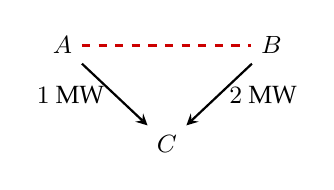
\begin{tikzpicture}[scale=0.78, every node/.style={font=\small}, >=stealth]
                \node (A) at (0,1.6) {$A$};
                \node (B) at (3.4,1.6) {$B$};
                \node (C) at (1.7,0) {$C$};

                \draw[red!80!black, dashed, thick] (A) -- (B);
                \draw[->, thick] (A) -- node[left] {$1$ MW} (C);
                \draw[->, thick] (B) -- node[right] {$2$ MW} (C);
            \end{tikzpicture}
        \end{column}
        \begin{column}{0.32\textwidth}
            \centering
            \textbf{$A \rightarrow C$ down}

            \vspace{0.35em}

            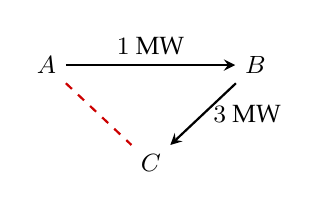
\begin{tikzpicture}[scale=0.78, every node/.style={font=\small}, >=stealth]
                \node (A) at (0,1.6) {$A$};
                \node (B) at (3.4,1.6) {$B$};
                \node (C) at (1.7,0) {$C$};

                \draw[->, thick] (A) -- node[above] {$1$ MW} (B);
                \draw[->, thick] (B) -- node[right] {$3$ MW} (C);
                \draw[red!80!black, dashed, thick] (A) -- (C);
            \end{tikzpicture}
        \end{column}
        \begin{column}{0.32\textwidth}
            \centering
            \textbf{$B \rightarrow C$ down}

            \vspace{0.35em}

            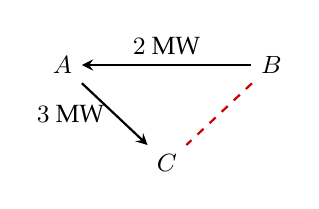
\begin{tikzpicture}[scale=0.78, every node/.style={font=\small}, >=stealth]
                \node (A) at (0,1.6) {$A$};
                \node (B) at (3.4,1.6) {$B$};
                \node (C) at (1.7,0) {$C$};

                \draw[<-, thick] (A) -- node[above] {$2$ MW} (B);
                \draw[->, thick] (A) -- node[left] {$3$ MW} (C);
                \draw[red!80!black, dashed, thick] (B) -- (C);
            \end{tikzpicture}
        \end{column}
    \end{columns}

    \begin{exampleblock}{Feasible Schedule}
        Since this load schedule is feasible in each contingency scenario (no transmission line is over capacity), the RTO approves. 
    \end{exampleblock}
\end{frame}

\begin{frame}
    \frametitle{Clearing Results}
    \small

    \begin{center}
    \resizebox{0.98\textwidth}{!}{%
    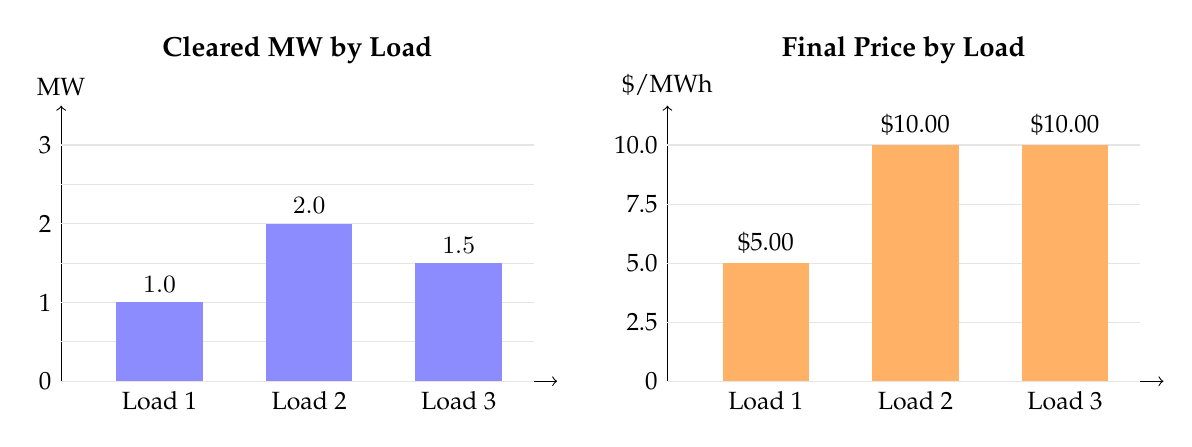
\begin{tikzpicture}[font=\small]
        % Left panel: allocated MW
        \begin{scope}[xshift=0cm]
            \node[font=\bfseries] at (3.0,4.2) {Cleared MW by Load};
            \draw[->] (0,0) -- (0,3.5) node[above] {MW};
            \draw[->] (0,0) -- (6.3,0);

            \foreach \y in {0,0.5,...,3} {
              \draw[gray!20] (0,\y) -- (6.0,\y);
            }
            \foreach \y/\label in {0/0,1/1,2/2,3/3} {
              \node[left] at (0,\y) {\label};
            }

            \fill[blue!45] (0.7,0) rectangle (1.8,1.0);
            \fill[blue!45] (2.6,0) rectangle (3.7,2.0);
            \fill[blue!45] (4.5,0) rectangle (5.6,1.5);

            \node[above] at (1.25,1.0) {$1.0$};
            \node[above] at (3.15,2.0) {$2.0$};
            \node[above] at (5.05,1.5) {$1.5$};

            \node[below] at (1.25,0) {Load 1};
            \node[below] at (3.15,0) {Load 2};
            \node[below] at (5.05,0) {Load 3};
        \end{scope}

        % Right panel: final price
        \begin{scope}[xshift=7.7cm]
            \node[font=\bfseries] at (3.0,4.2) {Final Price by Load};
            \draw[->] (0,0) -- (0,3.5) node[above] {\$/MWh};
            \draw[->] (0,0) -- (6.3,0);

            \foreach \y in {0,0.75,...,3} {
              \draw[gray!20] (0,\y) -- (6.0,\y);
            }
            \foreach \y/\label in {0/0,0.75/2.5,1.5/5.0,2.25/7.5,3/10.0} {
              \node[left] at (0,\y) {\label};
            }

            \fill[orange!60] (0.7,0) rectangle (1.8,1.5);
            \fill[orange!60] (2.6,0) rectangle (3.7,3.0);
            \fill[orange!60] (4.5,0) rectangle (5.6,3.0);

            \node[above] at (1.25,1.5) {\$5.00};
            \node[above] at (3.15,3.0) {\$10.00};
            \node[above] at (5.05,3.0) {\$10.00};

            \node[below] at (1.25,0) {Load 1};
            \node[below] at (3.15,0) {Load 2};
            \node[below] at (5.05,0) {Load 3};
        \end{scope}
    \end{tikzpicture}%
    }
    \end{center}

    \vspace{-0.4em}
    \begin{columns}[T,onlytextwidth]
        \begin{column}{0.28\textwidth}
            \centering
            \textbf{Optimal dispatch}
            \begin{center}
            \scriptsize
            \begin{tabular}{lc}
                \toprule
                Generator & MW \\
                \midrule
                Gen 1 ($A$) & 2.0 \\
                Gen 2 ($B$) & 2.0 \\
                Gen 3 ($C$) & 0.5 \\
                \bottomrule
            \end{tabular}
            \end{center}
        \end{column}
        \begin{column}{0.26\textwidth}
            \centering
            \textbf{Locational prices}
            \begin{center}
            \scriptsize
            \begin{tabular}{lc}
                \toprule
                Node & \$/MWh \\
                \midrule
                $A$ & 5.00 \\
                $B$ & 10.00 \\
                $C$ & 10.00 \\
                \bottomrule
            \end{tabular}
            \end{center}
        \end{column}
        \begin{column}{0.42\textwidth}
            \begin{exampleblock}{Takeaway}
                Locational prices can vary in a power grid due to transmission limits, known as congestion.
            \end{exampleblock}
        \end{column}
    \end{columns}
\end{frame}

%------------------------------------------------

\section{DA Clearing LP Formulation}

\begin{frame}
    \frametitle{DA LP Formulation}
    \small
 
    \begin{alertblock}{Objective (x = cleared MWh)}
        max $\text{ }\sum{\text{Load MWh } \times \text{Price}}$ - $\sum{\text{Gen MWh } \times \text{Price}}$
    \end{alertblock}

    \vspace{-0.4em}

    \textit{s.t.}

    \vspace{-0.5em}

    \begin{block}{Power Balance Constraint}
        MW Generated = MW Consumed across the grid (assume no loss)
    \end{block}

    \vspace{-0.6em}

    \begin{exampleblock}{Gen, Load Feasibility}
        Generators cleared in [min, max] range. Loads allocated $\leq$ Demand
    \end{exampleblock}

    \vspace{-0.6em}

    \begin{block}{Base-Case Thermal Constraints}
        Cleared solution does not result in overloaded transmission line
    \end{block}

    \vspace{-0.6em}

    \begin{exampleblock}{(N-1) Contingency Thermal Constraints}
        No transmission overload in any contingency scenario
    \end{exampleblock}
    
\end{frame}

%------------------------------------------------

\begin{frame}
    \frametitle{Financial Transmission Rights}
    \small

    \[
        \text{Payout} = (LMP_{\text{sink}} - LMP_{\text{source}})\times \text{Quantity}
    \]

    \begin{itemize}
        \item An FTR is a financial right on congestion between two nodes.
        \item Utilities and generators use FTRs to hedge uncertain nodal price differences.
        \item The auction clears awarded quantities $x_r$ subject to a Simultaneous Feasibility Test (SFT).
    \end{itemize}

    {\scriptsize
    \[
    \begin{aligned}
    -F_l^{\max}
    &\le
    \sum_{r\in\mathcal{R}} \big(PTDF^{(k)}_{l,t(r)} - PTDF^{(k)}_{l,o(r)}\big)x_r &\le F_l^{\max}
    \end{aligned}
    \]
    }

    \begin{block}{Takeaway 3}
        The RTO can only sell an FTR portfolio that remains feasible with the same transmission limits used in the Day-Ahead market.
    \end{block}
\end{frame}

%------------------------------------------------

\section{FTR Clearing LP Formulation}

\begin{frame}
\frametitle{FTR Clearing LP Formulation}

    \begin{alertblock}{Objective (x = cleared MWh)}
        max value of cleared FTR contracts
    \end{alertblock}

    \textit{s.t.}

    \begin{block}{Availability Constraint}
        Cleared quantity does not exceed number of available FTR contracts
    \end{block}
    \begin{exampleblock}{Base-Case Thermal Constraints}
        Cleared solution obeys full-grid thermal constraints
    \end{exampleblock}
    \begin{block}{(N-1) Contingency Thermal Constraints}
        Cleared solution obeys all contingency situations
    \end{block}
    
\end{frame}

%------------------------------------------------

\section{IEE 118-Bus Large-Scale Example}

\begin{frame}
    \frametitle{Data Collection}
    \small

    Great! Let's just run this on real grid data...

    \begin{alertblock}{\textit{FERC Order No.'s 643/833}}
        \textit{Requests for electronic copies of grid data are subject to approval by the Federal Energy Regulatory Commission and signature of NDAs}.
    \end{alertblock}

    \begin{itemize}
        \item Luckily - the IEEE has sample networks from the 60's available in the public domain.
        \item We use a software called PowerWorld to read these binaries and export \alert{.csv's} of \alert{bus}, \alert{branch}, \alert{generator} definitions.
        \item Powerworld also calculates \alert{shift factors} with transmission line characteristics from the model. 
    \end{itemize}
\end{frame}

%------------------------------------------------

\section{Results Analysis}

\begin{frame}
    \frametitle{Running the LP}
    \small

    \begin{center}
        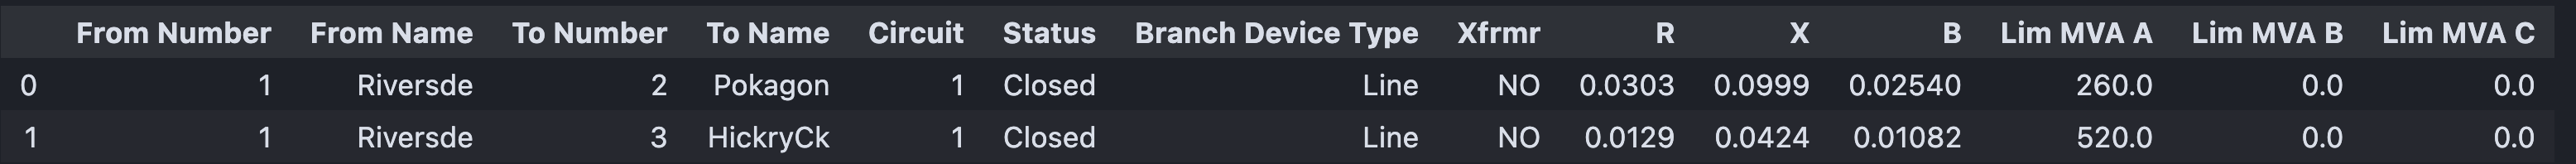
\includegraphics[width=1\textwidth]{assets/image_7.png}

        {\scriptsize Branch Definitions from PowerWorld}
    \end{center}

    \vspace{0.15em}

    \begin{columns}[T,onlytextwidth]
        \begin{column}{0.40\textwidth}
            \begin{block}{Run summary}
                \begin{enumerate}
                    \item Chose IEEE 118-bus model for substantial size
                    \item Produced random bid/offer stack due to lack of data
                    \item Gurobi solves resulting DA LP after 19 seconds
                    \item FTR LP solved $<$ 1s
                \end{enumerate}
            \end{block}
        \end{column}
        \begin{column}{0.56\textwidth}
            \raggedleft
            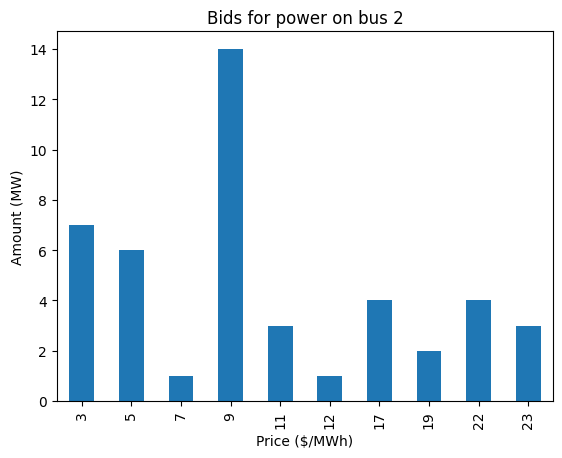
\includegraphics[width=0.7\linewidth,height=0.45\textheight,keepaspectratio]{assets/image_4.png}

            {\scriptsize Randomly generated bids for 1 bus}

            \vspace{0.45em}

            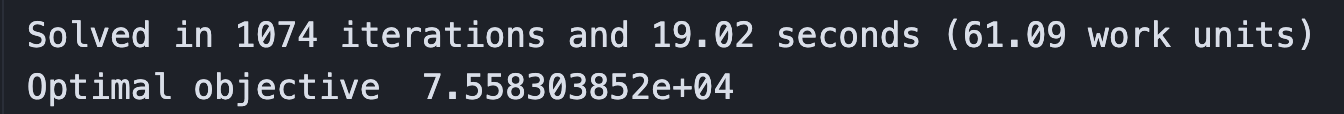
\includegraphics[width=0.98\linewidth,height=0.08\textheight,keepaspectratio]{assets/image_5.png}

            {\scriptsize Final Gurobi Solve Time of 19s}
        \end{column}
    \end{columns}

\end{frame}

\begin{frame}
    \frametitle{Results}
    \begin{center}
        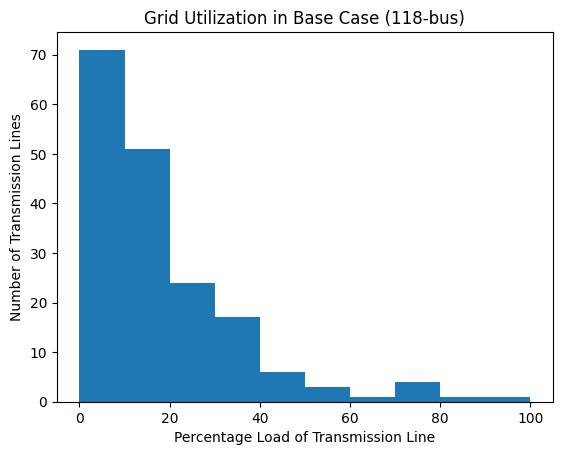
\includegraphics[width=0.6\textwidth]{assets/image_6.png}
    \end{center}

    \begin{block}{Low Utilization - good for reliability}
    There are however some high-load lines. This is where the RTO would build new infrastructure.
    \end{block}
\end{frame}

\begin{frame}
    \frametitle{Results}
    \begin{center}
        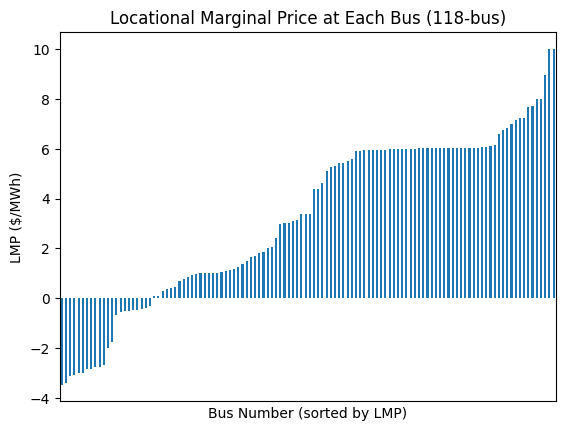
\includegraphics[width=0.615\textwidth]{assets/image_9.png}
    \end{center}
    \begin{block}{High LMP differences}
    Differences in LMP mainly come from the contingency analysis. Negative prices are also interesting!
    \end{block}
\end{frame}

%----------------------------------------------------------------------------------------
%\tCLOSING SLIDE
%----------------------------------------------------------------------------------------

\begin{frame}
    \frametitle{Solving this problem at scale}

    \small

    \begin{columns}[T,onlytextwidth]
        \begin{column}{0.36\textwidth}
            \begin{beamercolorbox}[wd=\linewidth,rounded=true,sep=0.9em]{block body}
                {\small\bfseries PJM in 2024\par}
                \vspace{0.5em}
                {\small
                \begin{itemize}
                    \item 1,436 generators
                    \item 6,000+ buses
                    \item 142,158 km of transmission lines
                    \item 800 TWh transmitted, about 53,000 Artemis II missions
                \end{itemize}
                \textit{PJM runs a similar LP every 5 minutes.}\par}
                \vspace{0.6em}
                {\scriptsize Source: \href{https://en.wikipedia.org/wiki/PJM_Interconnection}{Wikipedia: PJM Interconnection}}
            \end{beamercolorbox}
        \end{column}
        \begin{column}{0.60\textwidth}
            \centering
                \begin{tikzpicture}
                    \begin{axis}[
                        width=0.93\linewidth,
                        height=0.60\textheight,
                        ymode=log,
                        log basis y={10},
                        symbolic x coords={24,30,39,57,118,300},
                        xtick=data,
                        enlarge x limits=0.12,
                        xlabel={Network size (buses)},
                        ylabel={Solve time (s, log scale)},
                        ymajorgrids=true,
                        yminorgrids=true,
                        xmajorgrids=false,
                        minor grid style={gray!15},
                        major grid style={gray!30},
                        tick label style={font=\scriptsize},
                        x tick label style={font=\scriptsize},
                        label style={font=\scriptsize},
                        title style={font=\scriptsize},
                        title={Observed solve time on our machine (log scale)},
                        mark options={scale=0.9},
                    ]
                        \addplot[
                            very thick,
                            blue,
                            mark=*,
                        ] coordinates {
                            (24,0.06)
                            (30,0.12)
                            (39,0.12)
                            (57,1.59)
                            (118,21.33)
                            (300,1953.45)
                        };
                    \end{axis}
                \end{tikzpicture}
        \end{column}
    \end{columns}
\end{frame}

\begin{frame}[plain]
    \begin{center}
        {\Huge Thank you}

        
\includegraphics[width=0.25\textwidth]{assets/image_2.png}

    \end{center}
\end{frame}


% --------------- Appendix ------------------ %

\begin{frame}
    \frametitle{Power Flow v. Min Cost Flow}
    \small

    \begin{itemize}
        \item Power cannot be manually routed line-by-line; it spreads according to the electrical properties of the network.
        \item PTDFs (shift factors) measure how a 1 MW injection at one node and withdrawal at another loads each transmission line.
        \item The RTO must enforce thermal limits in the base case and after any single-line outage.
    \end{itemize}

    \begin{equation*}
        \mathrm{flow}_{l}
        =
        \sum_{s \in \mathcal{N}} PTDF_{l,s}\,\mathrm{inj}_{s}
    \end{equation*}

    \begin{alertblock}{Reliability requirement}
        The same dispatch must remain feasible under all monitored contingencies ($N$-$1$ security).
    \end{alertblock}
\end{frame}

\begin{frame}
    \frametitle{DA LP Formulation}
    \footnotesize

    \begin{align*}
        \max_{g,d}\quad
        & \sum_{d\in\mathcal D} p_d\, d_d \;-\; \sum_{g\in\mathcal G} c_g\, g_g \\[6pt]
        \text{s.t.}\quad
        & \sum_{g\in\mathcal G} g_g \;-\; \sum_{d\in\mathcal D} d_d \;=\; 0 \\[6pt]
        & g_g^{\min} \le g_g \le g_g^{\max}
        \qquad \forall g\in\mathcal G \\[6pt]
        & 0 \le d_d \le d_d^{\text{nom}}
        \qquad \forall d\in\mathcal D \\[6pt]
        & inj_s \;=\;
        \sum_{g:n(g)=s} g_g
        \;-\;
        \sum_{d:n(d)=s} d_d
        \qquad \forall s\in\mathcal N \\[6pt]
        & -F_l^{\max}
        \le
        \sum_{s\in\mathcal N} PTDF_{l,s}\,inj_s
        \le
        F_l^{\max}
        \qquad \forall l\in\mathcal L \\[6pt]
        & -F_l^{\max}
        \le
        \sum_{s\in\mathcal N} PTDF^{(k)}_{l,s}\,inj_s
        \le
        F_l^{\max}
        \qquad \forall (l,k)\in\mathcal C
\end{align*}

\begin{enumerate}
    \item Where $\mathcal G$, $\mathcal D$ are generators and loads
\end{enumerate}

\end{frame}

\begin{frame}
    \frametitle{LMP Calculation}
    \footnotesize
   
   \[
        \lambda
        := \text{dual variable of the power-balance constraint,}
        \]

        \[
        \mu_l^{\max},\ \mu_l^{\min}
        := \text{dual variables of }
        \sum_{s\in\mathcal N} PTDF_{l,s}\,inj_s \le F_l^{\max}
        \text{ and }
        \sum_{s\in\mathcal N} PTDF_{l,s}\,inj_s \ge -F_l^{\max},
        \]

        \[
        \mu_{l,k}^{\max},\ \mu_{l,k}^{\min}
        := \text{dual variables of }
        \sum_{s\in\mathcal N} PTDF^{(k)}_{l,s}\,inj_s \le F_l^{\max}
        \text{ and }
        \sum_{s\in\mathcal N} PTDF^{(k)}_{l,s}\,inj_s \ge -F_l^{\max}.
        \]

    \begin{align*}
        \mathrm{LMP}_i^{\text{base}}
        &=
        \lambda
        +
        \sum_{l\in\mathcal L}
        PTDF_{l,i}\,
        \bigl(\mu_l^{\max}+\mu_l^{\min}\bigr),
        \qquad \forall i\in\mathcal N, \\[6pt]
        \mathrm{LMP}_i
        &=
        -\left(
        \mathrm{LMP}_i^{\text{base}}
        +
        \sum_{(l,k)\in\mathcal C}
        PTDF^{(k)}_{l,i}\,
        \bigl(\mu_{l,k}^{\max}+\mu_{l,k}^{\min}\bigr)
        \right),
        \qquad \forall i\in\mathcal N.
    \end{align*}
\end{frame}

\begin{frame}
    \frametitle{FTR LP Formulation}
    \footnotesize

    \begin{align*}
        \max_{x}\quad
        & \sum_{r\in\mathcal R} p_r\,x_r \\[6pt]
        \text{s.t.}\quad
        & 0 \le x_r \le \bar q_r
        \qquad \forall r\in\mathcal R \\[6pt]
        & -F_l^{\max}
        \le
        \sum_{r\in\mathcal R}
        \left( PTDF_{l,t(r)} - PTDF_{l,o(r)} \right)x_r
        \le
        F_l^{\max}
        \qquad \forall l\in\mathcal L \\[6pt]
        & -F_l^{\max}
        \le
        \sum_{r\in\mathcal R}
        \left( PTDF^{(k)}_{l,t(r)} - PTDF^{(k)}_{l,o(r)} \right)x_r
        \le
        F_l^{\max}
        \qquad \forall l\in\mathcal L,\ \forall k\in\mathcal K
        \end{align*}
\end{frame}



%----------------------------------------------------------------------------------------

\end{document}
